\begin{appendices}
\chapter{Default incentives for different $\bm{\alpha}$}

Figures A.1-A.4 present the default incentives under different bargain power distributions from before and after the introduction of Eurobonds. The default decision $\hat{p}$ is dependent on the set of combinations of defaultable debt $d$, non-defaultable debt $e$ and output $y$. Two scenarios will be considered: i) an economy without and with Eurobonds for which both economies non-defaultable debt is set equal to zero ($e = 0$) ii) an economy without and with Eurobonds where both are at their non-defaultable debt limit, $e = 0$ and $e = 0.4$ respectively. For both panels the dark area represents the combinations of $(d,y)$ for which a government defaults and the white area the combinations for which it repays its debt.
\begin{figure}[H]
\caption{\textbf{Default decision for $\bm{\alpha = 0.55}$}}
    \centering
    \vspace{1mm}
     \resizebox{\columnwidth}{4.8cm}{%
   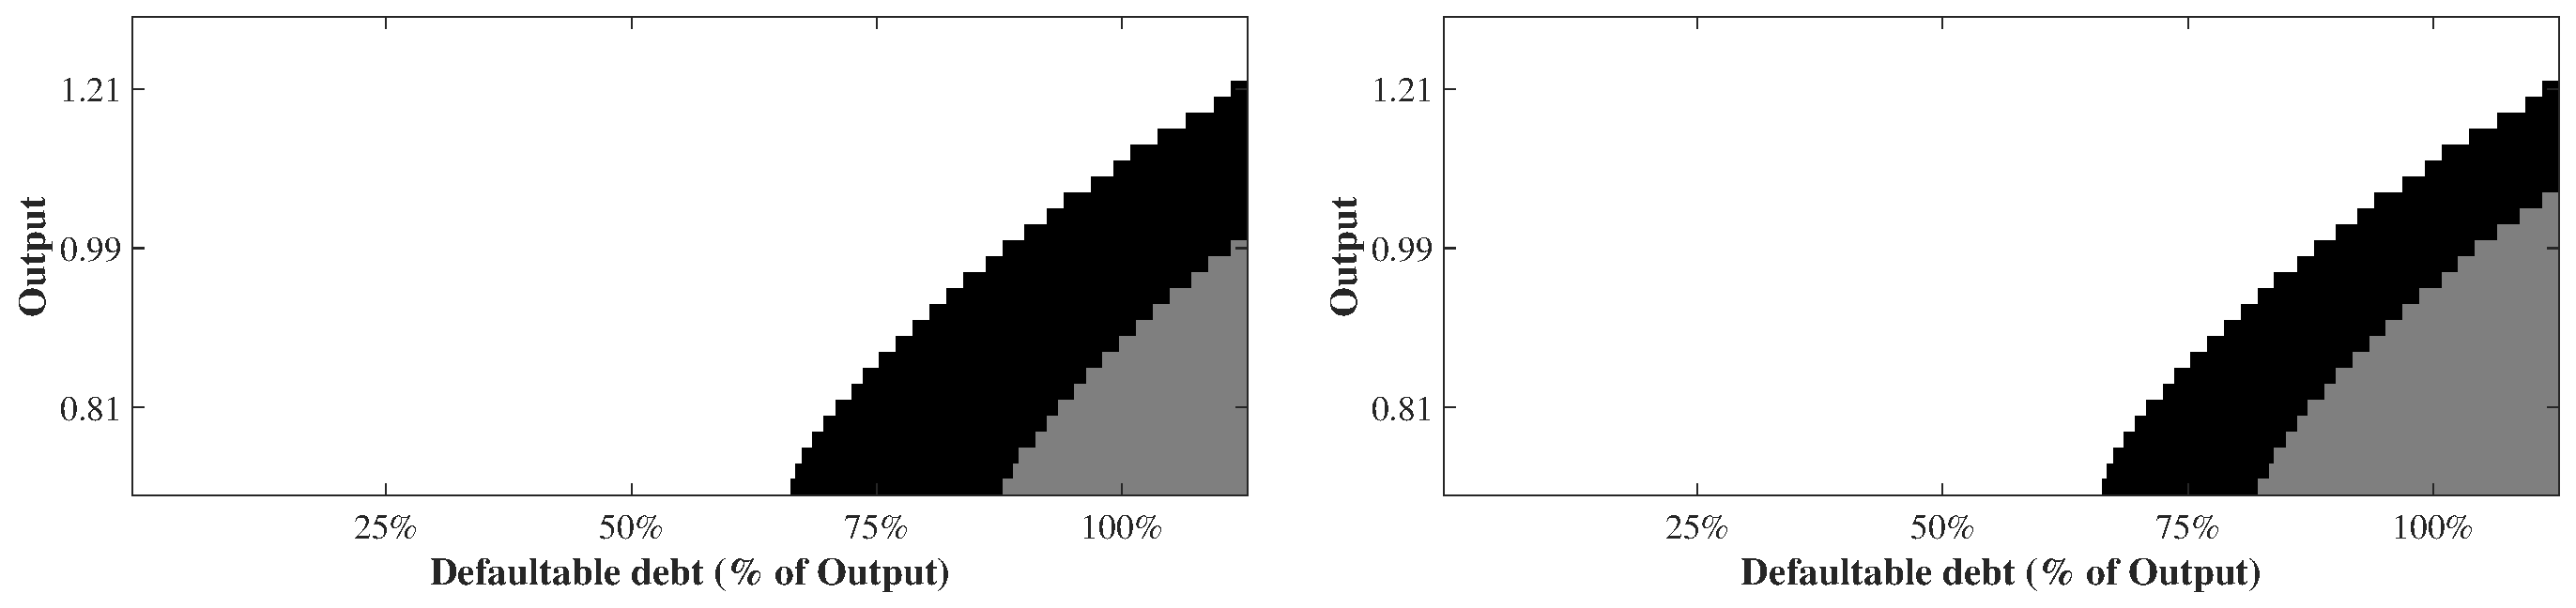
\includegraphics[scale=0.27]{default_decision_alpha55.eps}
    }
        \begin{tablenotes}
      \footnotesize
    Figure A.1 shows the default decision matrix for an economy without (black area) and an economy with Eurobonds (gray area). The left panel displays the decision where for both economies $e = 0$. The right panel shows the default decision where both economies are at their non-defaultable debt limit, $e = 0$ and $e = 0.4$ respectively.
    \end{tablenotes}
\end{figure}
\vspace{11mm} 
\begin{figure}[H]
\caption{\textbf{Default decision for $\bm{\alpha = 0.65}$}}
    \centering
    \vspace{1mm}
     \resizebox{\columnwidth}{4.6cm}{%
   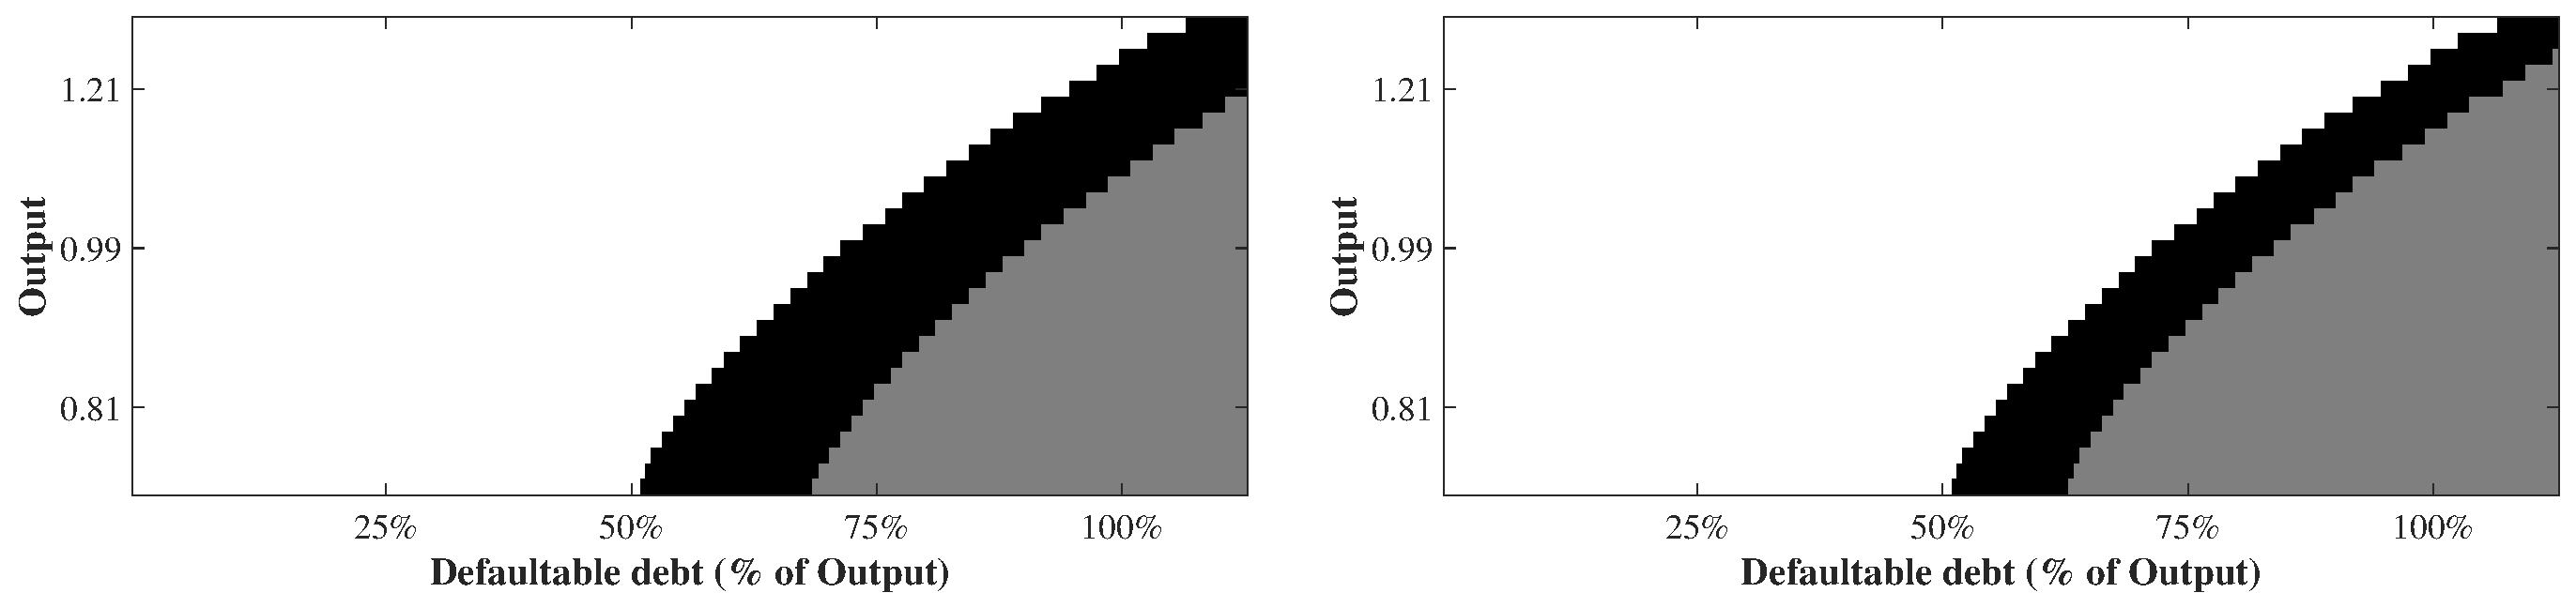
\includegraphics[scale=0.27]{default_decision_alpha65.eps}
    }
        \begin{tablenotes}
      \footnotesize
    Figure A.2 shows the default decision matrix for an economy without (black area) and an economy with Eurobonds (gray area). The left panel displays the decision where for both economies $e = 0$. The right panel shows the default decision where both economies are at their non-defaultable debt limit, $e = 0$ and $e = 0.4$ respectively.
    \end{tablenotes}
\end{figure}

\begin{figure}[H]
\caption{\textbf{Default decision for $\bm{\alpha = 0.75}$}}
    \centering
    \vspace{1mm}
     \resizebox{\columnwidth}{4.6cm}{%
   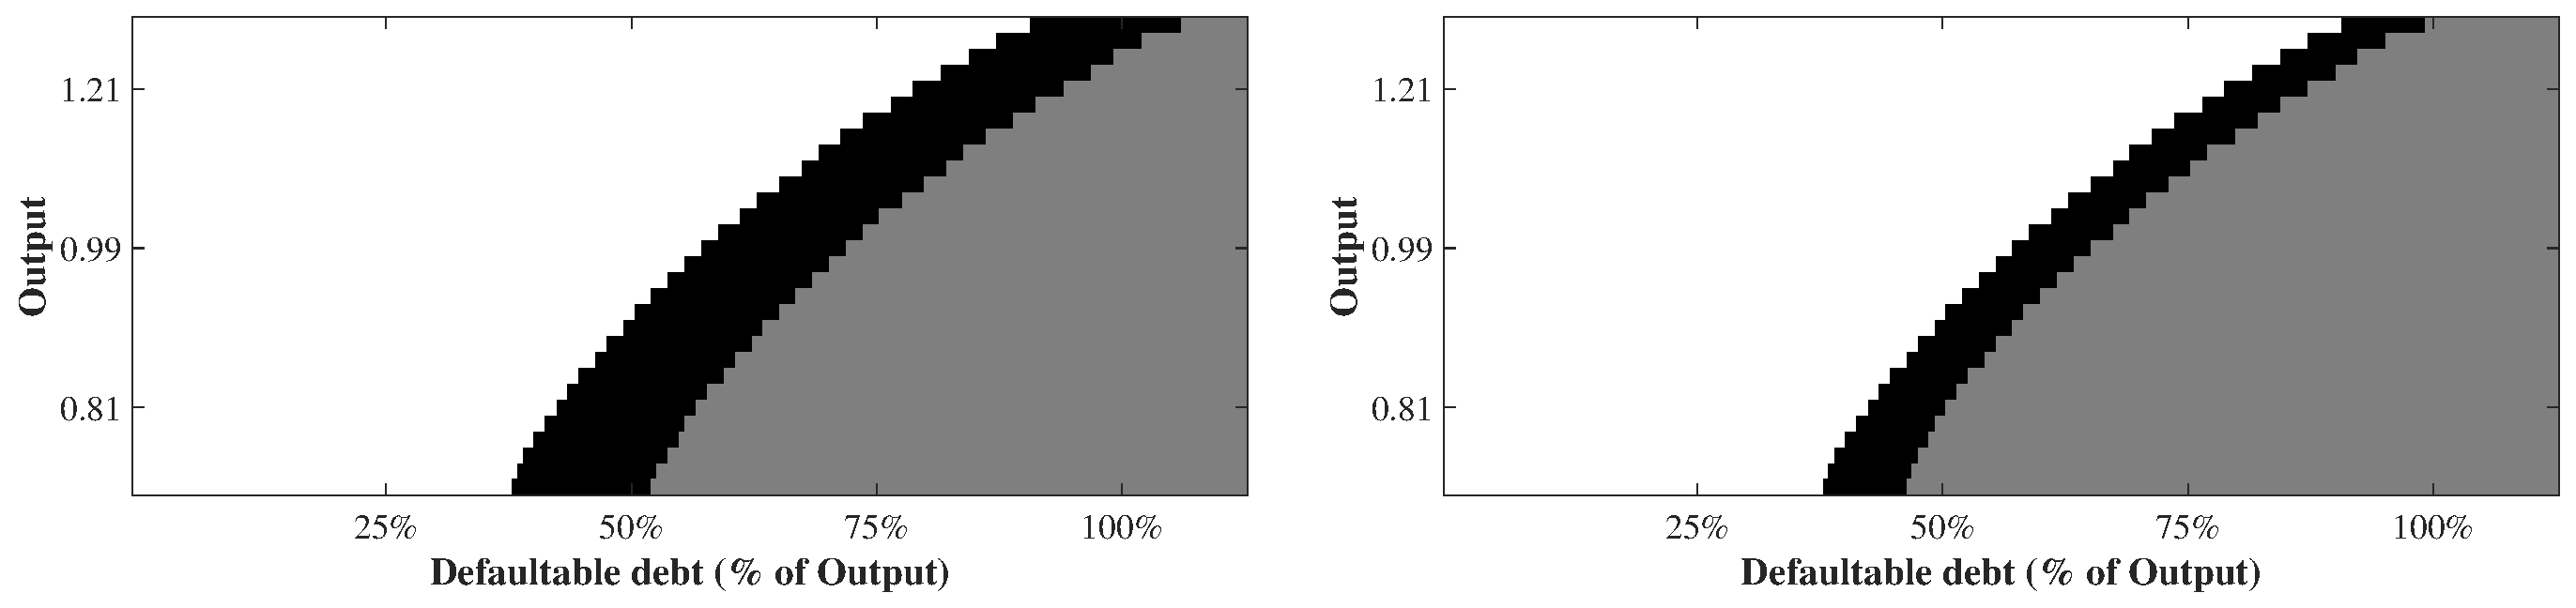
\includegraphics[scale=0.27]{default_decision_alpha75.eps}
    }
        \begin{tablenotes}
      \footnotesize
    Figure A.3 shows the default decision matrix for an economy without (black area) and an economy with Eurobonds (gray area). The left panel displays the decision where for both economies $e = 0$. The right panel shows the default decision where both economies are at their non-defaultable debt limit, $e = 0$ and $e = 0.4$ respectively.
    \end{tablenotes}
\end{figure}

\begin{figure}[H]
\caption{\textbf{Default decision for $\bm{\alpha = 1}$}}
    \centering
    \vspace{1mm}
     \resizebox{\columnwidth}{4.6cm}{%
   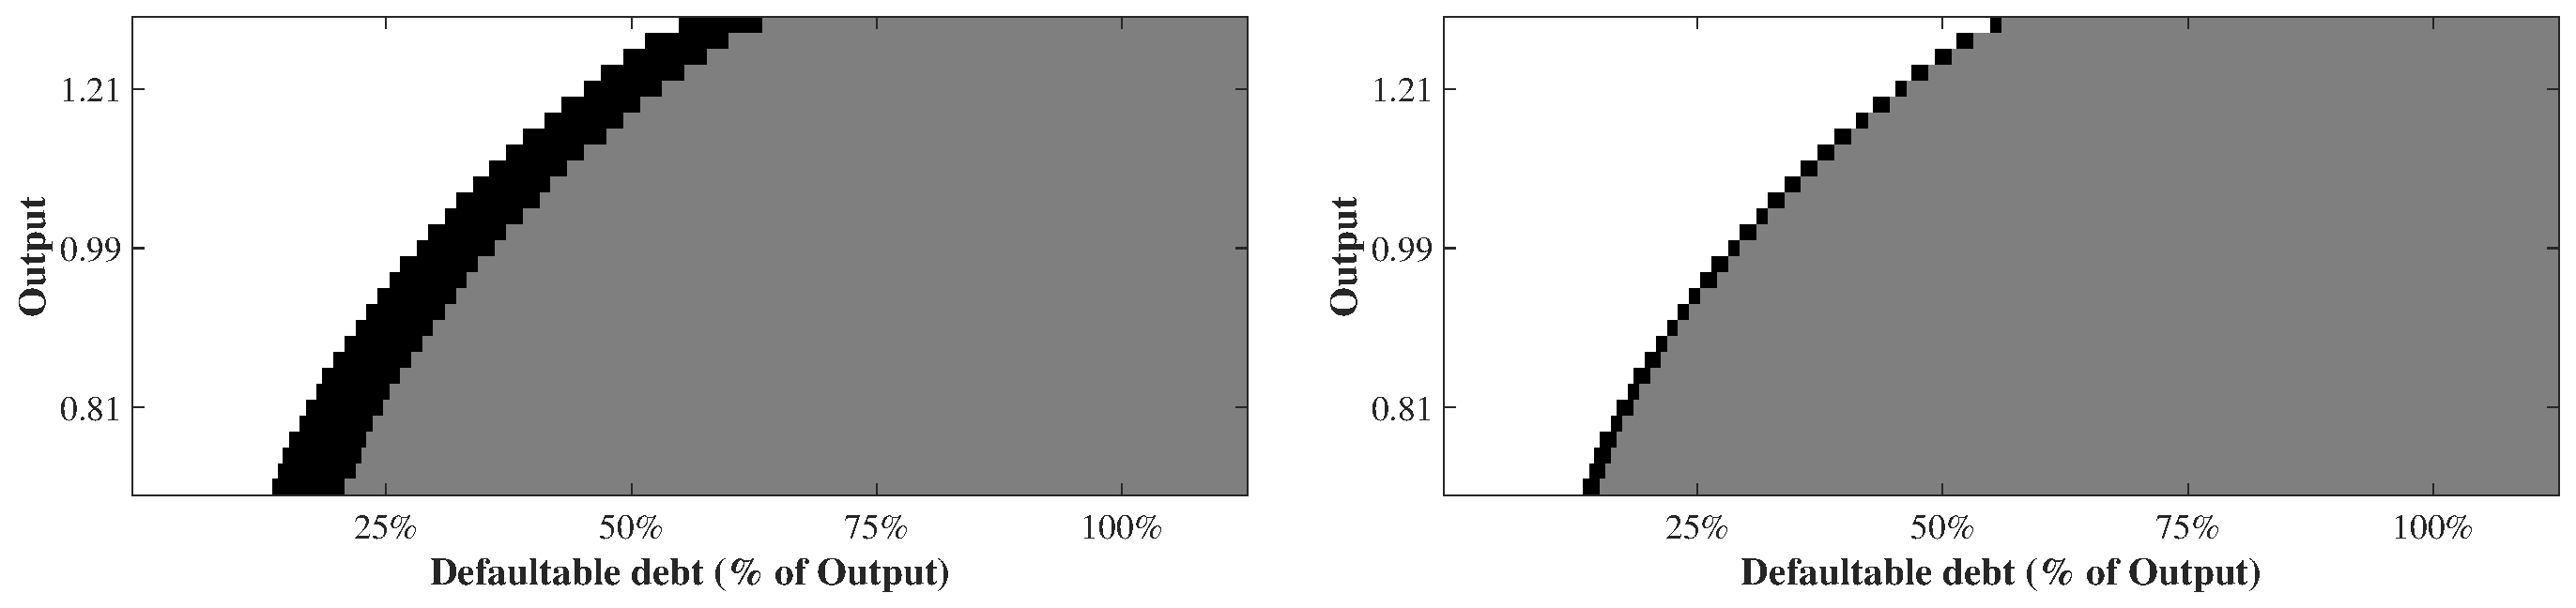
\includegraphics[scale=0.27]{default_decision_alpha1.eps}
    }
        \begin{tablenotes}
      \footnotesize
    Figure A.4 shows the default decision matrix for an economy without (black area) and an economy with Eurobonds (gray area). The left panel displays the decision where for both economies $e = 0$. The right panel shows the default decision where both economies are at their non-defaultable debt limit, $e = 0$ and $e = 0.4$ respectively.
    \end{tablenotes}
\end{figure}

\end{appendices}

\begin{appendices}
\chapter{Step-by-step guide to replicating the results}
This appendix goes over the step-by-step replication of the dissertation's results. All figures and tables are generated in \texttt{Matlab} and the \texttt{.m-files} to solve the model and run the simulations are based on Uribe \& Schmitt-Grohé's code which is available online\footnote{\url{http://www.columbia.edu/~mu2166/book/sovereign_debt/}}.\\

Before running the code, two comments should be taken into consideration. First of all, to improve \texttt{Matlab}'s efficiency in solving the model, defaultable debt and non-defaultable debt are treated jointly. This means that government debt is represented by a "bundle" of regular debt and Eurobonds. By doing so, we increase the computational efficiency in the maximization routines by treating the problem as a 2-dimensional instead of a 3-dimensional problem. A second remark to take into consideration is that solving for every calibration of the model can take up to 6 days or more, depending on your hardware specifications. The baseline model alone with Eurobonds can take 20 hours or more to solve. The smaller the grid size of the model, the lower the computation time and vice versa. All original \texttt{.mat-files} are available on request to immediately replicate the results from Step 3 (cf. infra).\\

To generate the results, the steps below need to be performed. It is imperative that between all \texttt{.m-files} the same names are used for the \texttt{.mat-files} in which the different solutions are stored. Certain \texttt{.m-files} require multiple inputs for which all names need to be adjusted accordingly. 
\begin{itemize}
    \item \textbf{Step 1:} Run \texttt{tpm.m} to generate the output grid and the transition matrix. The resulting \texttt{.mat-file} will be used as input for Step 2.
    \item \textbf{Step 2:} Run \texttt{egr\_nondef\_final.m} to solve the model through Value Function Iteration. This step needs to be repeated for every change made to the baseline calibration.
    \item \textbf{Step 3:} All tables and figures are generated by separate \texttt{.m-files}. Every first file in the following steps uses the generated \texttt{.mat-file} from Step 2.
    \begin{itemize}
        \item All tables are generated by running \texttt{simu\_regular.m} and \texttt{statistics.m} in this order. This step needs to be repeated for every different calibration.
        \item Figure \ref{fig:default decision} and Figures A.1-A.4 are generated by \texttt{Default\_decision.m} and uses 2 \texttt{.mat-files} as input: the first with Eurobonds and the second without Eurobonds.
        \item Figure \ref{fig:intro} is generated by running \texttt{simu\_intro.m} and \texttt{Introduction.m} in this order.
        \item Figure \ref{fig:default_episode} is generated by running \texttt{simur\_regular.m} and \texttt{default\_episode.m} in this order.
        \item Figure \ref{fig:intro_comp} is generated by running \texttt{simu\_intro.m} and \texttt{intro\_comp.m} in this order. The file \texttt{simu\_intro.m} needs to be run five times for each separate calibration.
        \item Figure \ref{fig:intro_debtrule} is generated by running \texttt{simu\_intro.m} and \texttt{intro\_comp\_debtrule.m} in this order. The file \texttt{simu\_intro.m} needs to be run four times for each separate calibration.
        \item Figure 3.6 and 3.7 are generated by running \texttt{multiplicity.m} which uses two \texttt{.mat-files} as input: the standard baseline model and the bad equilibrium model.
    \end{itemize}
\end{itemize}
\end{appendices}


